%%%%%%%%%%%%%%%%%%%%%%%%%%%%%%%%%%%%%%%%%%%%%%%%%%%%%%%%%%%%%%%%%%%%%%%%%%%%%%%%%%%%%%%
%%%%%%%%%%%%%%%%%%%%%%%%%%%%%%%%%%%%%%%%%%%%%%%%%%%%%%%%%%%%%%%%%%%%%%%%%%%%%%%%%%%%%%%%%%%%%%%%%%%%%%%%
%%%%%%%%%%%%%%%%%%%%%%%%%%%%%%%%%%%%%%%%%%%%%%%%%%%%%%%%%%%%%%%%%%%%%%%%%%%%%%%%%%%%%%%%%%%%%%%%%%%%%%%%
\chapter[Schéma fonctionnels]{Schémas fonctionnels et graphes de fluence\label{chap-schemabloc}}
%%%%%%%%%%%%%%%%%%%%%%%%%%%%%%%%%%%%%%%%%%%%%%%%%%%%%%%%%%%%%%%%%%%%%%%%%%%%%%%%%%%%%%%
%%%%%%%%%%%%%%%%%%%%%%%%%%%%%%%%%%%%%%%%%%%%%%%%%%%%%%%%%%%%%%%%%%%%%%%%%%%%%%%%%%%%%%%%%%%%%%%%%%%%%%%%
%%%%%%%%%%%%%%%%%%%%%%%%%%%%%%%%%%%%%%%%%%%%%%%%%%%%%%%%%%%%%%%%%%%%%%%%%%%%%%%%%%%%%%%%%%%%%%%%%%%%%%%%

\minitoc
\newpage
%%%%%%%%%%%%%%%%%%%%%%%%%%%%%%%%%%%%%%%%%%%%%%%%%%%%%%%%%%%%%%%%%%%%%%%%%%%%%%%%%%%%%%%%%%%%%%%%%%%%%%%%
%%%%%%%%%%%%%%%%%%%%%%%%%%%%%%%%%%%%%%%%%%%%%%%%%%%%%%%%%%%%%%%%%%%%%%%%%%%%%%%%%%%%%%%
\section{Introduction}
%%%%%%%%%%%%%%%%%%%%%%%%%%%%%%%%%%%%%%%%%%%%%%%%%%%%%%%%%%%%%%%%%%%%%%%%%%%%%%%%%%%%%%%%%%%%%%%%%%%%%%%%
%%%%%%%%%%%%%%%%%%%%%%%%%%%%%%%%%%%%%%%%%%%%%%%%%%%%%%%%%%%%%%%%%%%%%%%%%%%%%%%%%%%%%%%
Dans ce chapitre, nous allons introduire un outil graphique pour faciliter 
la représentation des relations mathématiques entre les différents 
éléments constituants un \gls{slci}. Cet outil est le \textbf{schéma fonctionnel} ou 
également appelé \textbf{schéma-bloc}. Les schémas fonctionnels nous seront très 
utiles pour l'étude des systèmes asservis. Nous introduirons une algèbre de blocs permettant
de réduire les schémas-blocs de grande taille. Nous aborderons également le cas des entrées multiples. 

Dans une dernière partie nous introduirons 
les graphes de fluence, comme présenté dans~\cite{Ostertag}. Ces derniers 
sont moins utilisés pour l'étude des \gls{slci}, et peuvent donc être négligés 
dans une première lecture, l'algèbre qui lui est associée s'avère cependant bien plus 
éfficace et pourra être utilisée dans d'autres 
applications (ex : éléctronique, réseaux de neurones).


%%%%%%%%%%%%%%%%%%%%%%%%%%%%%%%%%%%%%%%%%%%%%%%%%%%%%%%%%%%%%%%%%%%%%%%%%%%%%%%%%%%%%%%%%%%%%%%%%%%%%%%%
%%%%%%%%%%%%%%%%%%%%%%%%%%%%%%%%%%%%%%%%%%%%%%%%%%%%%%%%%%%%%%%%%%%%%%%%%%%%%%%%%%%%%%%
\section{\'Eléments de base des schémas fonctionnels}
%%%%%%%%%%%%%%%%%%%%%%%%%%%%%%%%%%%%%%%%%%%%%%%%%%%%%%%%%%%%%%%%%%%%%%%%%%%%%%%%%%%%%%%%%%%%%%%%%%%%%%%%
%%%%%%%%%%%%%%%%%%%%%%%%%%%%%%%%%%%%%%%%%%%%%%%%%%%%%%%%%%%%%%%%%%%%%%%%%%%%%%%%%%%%%%%
Les schémas fonctionnels sont composés de quatre éléments de base:
\textbf{les flèches, les blocs, les comparateurs et sommateurs et les points de prélèvement}
%\begin{itemize}
%    \item les flèches.
%    \item les blocs.
%    \item les comparateurs et sommateurs.
%    \item les points de prélèvement.
%\end{itemize}

%\newpage
%%%%%%%%%%%%%%%%%%%%%%%%%%%%%%%%%%%
\paragraph{Flèche}
%%%%%%%%%%%%%%%%%%%%%%%%%%%%%%%%%%%
Les flèches donnent la direction de l'information (i.e du signal) au sein du schéma-blocs. 
Elles peuvent être ornées de la grandeur mathématique qui leurs sont associée. 
Celles-ci peuvent être des grandeurs temporelles ou dans le domaine de Laplace. 
\begin{center}
\tikzsetnextfilename{sb_fleche-chap1_ext}
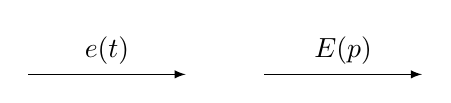
\begin{tikzpicture}
    \draw[-latex] (-3,0) -- (-1,0) node[midway,above] {$e(t)$};
    \draw[-latex] (0,0) -- (2,0) node[midway,above] {$E(p)$};
\end{tikzpicture}    
\end{center}
Cependant, nous nous limiterons à l'usage de ces schémas fonctionnelles pour la représentation
de grandeur dans le domaine de Laplace.

Pour alléger la notation dans ce chapitre, nous omettrons 
très souvent la variable $p$ des grandeurs dans le domaine de Laplace désignées par une majuscule.

\newpage
%%%%%%%%%%%%%%%%%%%%%%%%%%%%%%%%%%%
\paragraph{Bloc}
%%%%%%%%%%%%%%%%%%%%%%%%%%%%%%%%%%%

Le bloc est la représentation d'une fonction de transfert entre deux grandeurs dans le domaine de Laplace.
Par exemple, la relation entre l'entrée $E$ et la sortie $S$ définit par la fonction de transfert $H$
qui s'écrit formellement, 
\begin{bequation}[ams align]
S = HE,\label{eq-ES}
\end{bequation}
est équivalente au schéma fonctionnel\footnote{Les schémas-blocs de ce document ont tous 
étaient réalisés avec les macros Ti\emph{k}Z (\verb?schemabloc?) écrit par R. Papanicola\cite{schemabloc}. 
\`A noter que des macros Ti\emph{k}Z (\verb?gfluence?) pour représenter les graphes de fluence 
de ce même chapitre, ont était fortement inspiré par ce même auteur.} 
suivant:

\begin{center}
\tikzsetnextfilename{sb_bloc-chap1_ext}
\begin{tikzpicture}
    \sbEntree{E1}
    \sbBloc[3]{B1}{$H$}{E1}
        \sbRelier[$E$]{E1}{B1}
    \sbSortie[3]{S1}{B1}
        \sbRelier[$S$]{B1}{S1}
\end{tikzpicture}    
\end{center}


%%%%%%%%%%%%%%%%%%%%%%%%%%%%%%%%%%%
\paragraph{Comparateur/Sommateur :}
%%%%%%%%%%%%%%%%%%%%%%%%%%%%%%%%%%%

Les comparateurs ou sommateurs permettent de représenter des opérations 
simples entre différentes grandeurs.
Nous parlerons respectivement de comparateur ou de sommateur dans le cas 
d'une différence ou d'une somme entre deux grandeurs. 


Par exemple, la relation 
$$
S = E_1-E_2 
$$
est équivalente au comparateur suivant :
\begin{center}
\tikzsetnextfilename{sb_comp-chap1_ext}
    \begin{tikzpicture}
        \coordinate (pt) at (0,-1);
        \sbEntree{E1}
        \sbComp[4.5]{comp}{E1}
        \sbRelier[$E_1$]{E1}{comp}
        \sbSortie[2.5]{S}{comp}
        \sbRelier[$S$]{comp}{S}
        \draw[-latex] (comp|-0,-1.5) -- (comp.south) node[midway,left] {$E_2$};
    \end{tikzpicture}
\end{center}

De même la somme de deux grandeurs,
$$                                                                                                                            
S = E_1+E_2                                                                                                          
$$
est équivalente au sommateur suivant :
\begin{center}
\tikzsetnextfilename{sb_somm-chap1_ext}
    \begin{tikzpicture}
        \coordinate (pt) at (0,-1);
        \sbEntree{E1}
        \sbSumb[4.5]{comp}{E1}
        \sbRelier[$E_1$]{E1}{comp}
        \sbSortie[2.5]{S}{comp}
        \sbRelier[$S$]{comp}{S}
        \draw[-latex] (comp|-0,-1.5) -- (comp.south) node[midway,left] {$E_2$};
    \end{tikzpicture}
\end{center}

%%%%%%%%%%%%%%%%%%%%%%%%%%%%%%%%%%%
\paragraph{Point de prélèvement}
%%%%%%%%%%%%%%%%%%%%%%%%%%%%%%%%%%%

Un point de prélèvement (ou point de dérivation ou encore jonction) 
est un point d'une flèche où une information est prélevée ne modifiant pas sa valeur.
Par exemple, la jonction suivante (représentée par un point) donne lieu à deux branches auxquelles sont
associées la même grandeur $S$.

\begin{center}
\tikzsetnextfilename{sb_point-chap1_ext}
    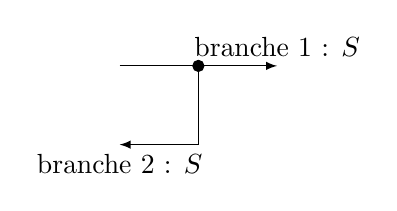
\begin{tikzpicture} 
    \draw[fill=black] (1,0) circle[radius=2.0pt];
    \draw[-latex] (0, 0) -- (2, 0) node[above] {branche 1 : $S$};
    \draw         (1, 0) -- (1,-1);
    \draw[-latex] (1,-1) -- (0,-1) node[below] {branche 2 : $S$};
    \end{tikzpicture}
\end{center}

Dans cette configuration, la branche 1 est dite \og direct\fg et la branche 2 est dite de \og retour\fg.

%%%%%%%%%%%%%%%%%%%%%%%%%%%%%%%%%%%%%%%%%%%%%%%%%%%%%%%%%%%%%%%%%%%%%%%%%%%%%%%%%%%%%%%
%%%%%%%%%%%%%%%%%%%%%%%%%%%%%%%%%%%%%%%%%%%%%%%%%%%%%%%%%%%%%%%%%%%%%%%%%%%%%%%%%%%%%%%%%%%%%%%%%%%%%%%%
\section{Transformation des schémas fonctionnels}
%%%%%%%%%%%%%%%%%%%%%%%%%%%%%%%%%%%%%%%%%%%%%%%%%%%%%%%%%%%%%%%%%%%%%%%%%%%%%%%%%%%%%%%
%%%%%%%%%%%%%%%%%%%%%%%%%%%%%%%%%%%%%%%%%%%%%%%%%%%%%%%%%%%%%%%%%%%%%%%%%%%%%%%%%%%%%%%%%%%%%%%%%%%%%%%%

%%%%%%%%%%%%%%%%%%%%%%%%%%%%%%%%%%%%%%%%%%%%%%%%%%%%%%%%%%%%%%%%%%%%%%%%%%%%%%%%%%%%%%%
\subsection{Réduction de schéma-bloc}
%%%%%%%%%%%%%%%%%%%%%%%%%%%%%%%%%%%%%%%%%%%%%%%%%%%%%%%%%%%%%%%%%%%%%%%%%%%%%%%%%%%%%%%

%%%%%%%%%%%%%%%%%%%%%%%%%%%%%%%%%%%%%%%%%%
\paragraph{Blocs en série / produit}
%%%%%%%%%%%%%%%%%%%%%%%%%%%%%%%%%%%%%%%%%%
Lorsque les blocs sont placés en série, la fonction de transfert 
entre la sortie et l'entrée globale est le produit des fonctions de transfert mis en jeu.
Par exemple, les deux schémas fonctionnels suivants sont équivalents.

\begin{center}
\tikzsetnextfilename{sb_reduc_serie_1-chap1_ext}
    \begin{tikzpicture} 
    \sbEntree{E1}
    \sbBloc[3]{B1}{$H_1$}{E1}
        \sbRelier[$E$]{E1}{B1}
    \sbBloc[3]{B2}{$H_2$}{B1}
        \sbRelier{B1}{B2}
    \sbBloc[3]{B3}{$H_3$}{B2}
        \sbRelier{B2}{B3}
    \sbSortie[3]{S1}{B3}
        \sbRelier[$S$]{B3}{S1}
        \node at (B2|-0,-1) {\rotatebox{90}{\LARGE$\equiv$}};
    \end{tikzpicture}

\tikzsetnextfilename{sb_reduc_serie_2-chap1_ext}
    \begin{tikzpicture} 
    \sbEntree{E1}
        \sbBloc[3]{B1}{$H=H_1H_2H_3$}{E1}
        \sbRelier[$E$]{E1}{B1}
    \sbSortie[3]{S1}{B1}
        \sbRelier[$S$]{B1}{S1}
    \end{tikzpicture}
\end{center}

Nous laissons au lecteur la démonstration triviale à partir des relations mathématiques.


%%%%%%%%%%%%%%%%%%%%%%%%%%%%%%%%%%%%%%%%%%%%%%%%%%%%%%%%%%%%%%%%%%%%%%%%%%%%%%%%%%%%%%%
\paragraph{Blocs en parallèle} 
%%%%%%%%%%%%%%%%%%%%%%%%%%%%%%%%%%%%%%%%%%%%%%%%%%%%%%%%%%%%%%%%%%%%%%%%%%%%%%%%%%%%%%%

Lorsque les blocs sont placés en parallèle, la fonction de transfert 
entre la sortie et l'entrée globale est la somme des fonctions de transfert mis en jeu.
Par exemple, les deux schémas fonctionnels suivants sont équivalents.

\begin{center}
\tikzsetnextfilename{sb_reduc_para_1-chap1_ext}
    \begin{tikzpicture} 
    \sbEntree{E1}
    \sbBloc[6]{B1}{$H_1$}{E1}
    \sbRelier{E1}{B1}
    \sbDecaleNoeudy[-4]{B1}{r1}
    \sbBloc[-1.6]{B2}{$H_2$}{r1}
    \sbRelieryx{E1-B1}{B2.west}
    \sbDecaleNoeudy[4]{B1}{r2}
    \sbBloc[-1.6]{B3}{$H_3$}{r2}
    \sbRelieryx{E1-B1}{B3.west}
    \sbCompSum[5]{C1}{B1}{+}{+}{+}{ }
    \sbRelier{B1}{C1}
    \sbRelierxy{B2}{C1}
    \sbRelierxy{B3}{C1}
    \sbSortie[3]{S1}{C1}
    \sbRelier[$S$]{C1}{S1}
    \node at (E1|-2.0,0.35) {$E$};
    \node at (B3|-0,-2.75) {\rotatebox{90}{\LARGE$\equiv$}};
%    \draw[fill=black] (1.325,0) circle[radius=2.0pt];
    \end{tikzpicture}

\tikzsetnextfilename{sb_reduc_para_2-chap1_ext}
    \begin{tikzpicture} 
      \sbEntree{E1}
    \sbBloc[3]{B1}{$H=H_1+H_2+H_3$}{E1}
    \sbRelier[$E$]{E1}{B1}
    \sbSortie[3]{S1}{B1}
    \sbRelier[$S$]{B1}{S1}
    \end{tikzpicture}
\end{center}

La démonstration est également triviale.

%%%%%%%%%%%%%%%%%%%%%%%%%%%%%%%%%%%%%%%%%%%%%%%%%%%%%%%%%%%%%%%%%%%%%%%%%%%%%%%%%%%%%%%
\paragraph{La boucle de contre-réaction (positive ou négative)\label{sec-boucle}}
%%%%%%%%%%%%%%%%%%%%%%%%%%%%%%%%%%%%%%%%%%%%%%%%%%%%%%%%%%%%%%%%%%%%%%%%%%%%%%%%%%%%%%%

La boucle de contre-réaction\footnote{\og Positive or negative feedback\fg, chez nos 
collègues anglophones.} peut 
être réduite à une simple fonction de transfert.
Considérons un système définit par le schéma-bloc ci-dessous, composé 
des différents élements de bases.

\begin{center}
    \tikzsetnextfilename{boucle-chap1_ext}
    \begin{tikzpicture}
    \sbEntree{E}
    \sbCompSum[5.0]{comp}{E}{}{\pm}{+}{}
        \sbRelier[$E$]{E}{comp}
        \sbBloc[3.5]{B}{$H_1$}{comp}
        \sbRelier[$\epsilon$]{comp}{B}
        \sbSortie[5.0]{S}{B}
        \sbRelier[$S$]{B}{S}
    \sbDecaleNoeudy[4]{B}{r1}
    \sbBlocr[-1.6]{B2}{$H_2$}{r1}
    \sbRelieryx{B-S}{B2}
        \sbRelierxy[$M$]{B2}{comp}
\end{tikzpicture}
\end{center}
Notons l'utilisation du symbole $\pm$ pour envisager à la fois les 
comparateurs et sommateurs.

Déterminons la relation entre l'entrée $E$ et la sortie $S$ de ce système.
Pour celà réécrivons les relations linéaires simples issus de ce schéma-bloc.
On sait que :
\begin{align}
    \epsilon&=E\pm M \label{eq-fb.1}\\
    M&=H_2S       \label{eq-fb.2}\\
    S&=H_1\epsilon \label{eq-fb.3}
\end{align}
Introduisons l'\cref{eq-fb.2} dans~(\ref{eq-fb.1}) et le résulat ainsi obtenu dans~(\ref{eq-fb.3}):
\begin{align*}
    \epsilon&=E\pm H_2S \\
     S&=H_1\big(E\pm H_2S\big) \\
     S&=H_1E\pm H_1H_2S
\end{align*}
Regroupons les termes dépendant de la sortie ensemble pour déterminer 
la relation entre l'entrée et la sortie.

\begin{align*}
    S\big(1\mp H_1H_2\big)&=H_1E 
\end{align*}

On obtient alors la formule de Black\footnote{\index{Black, Harold}Harold Stephen Black (1898-1983) ingénieur, 
électronicien américain.}, 
reliant la sortie est l'entrée d'une boucle de contre-réaction :
\begin{bequation}[ams align]
    S&=\dfrac{H_1}{1\mp H_1H_2}E
\end{bequation}

Notons l'inversion du signe du dénominateur de la formule 
selon que la boucle est positive ou négative.

La boucle de contre-réaction est donc équivalente au schéma-bloc simplifié suivant :
\begin{center}
    \tikzsetnextfilename{boucle_eq-chap1_ext}
    \begin{tikzpicture}
        \sbEntree{E1}
        \sbBloc[3]{B1}{$\dfrac{H_1}{1\mp H_1H_2}$}{E1}
        \sbRelier[$E$]{E1}{B1}
        \sbSortie[3]{S1}{B1}
        \sbRelier[$S$]{B1}{S1}
    \end{tikzpicture}    
\end{center}


%%%%%%%%%%%%%%%%%%%%%%%%%%%%%%%%%%%%%%%%%%%%%%%%%%%%%%%%%%%%%%%%%%%%%%%%%%%%%%%%%%%%%%%%%%%%%%%%%%%%%%%%
\paragraph{Boucle de contre-réaction unitaire}
%%%%%%%%%%%%%%%%%%%%%%%%%%%%%%%%%%%%%%%%%%%%%%%%%%%%%%%%%%%%%%%%%%%%%%%%%%%%%%%%%%%%%%%%%%%%%%%%%%%%%%%%

Une boucle de contre-réaction unitaire est une boucle de contre-réaction sans 
fonction de transfert de retour (ex: dans le cas présenté précedemment $H_2=1$).

\begin{center}
    \tikzsetnextfilename{boucle_uni-chap1_ext}
    \begin{tikzpicture}
    \sbEntree{E}
    \sbComp[5.0]{comp}{E}
        \sbRelier[$E$]{E}{comp}
        \sbBloc[3.0]{B}{$H_1$}{comp}
        \sbRelier[$\epsilon$]{comp}{B}
        \sbSortie[5.0]{S}{B}
        \sbRelier[$S$]{B}{S}
    \sbRenvoi{B-S}{comp}{}
\end{tikzpicture}
\end{center}

La formule de Black se simplifie alors de la façon suivante :
\begin{bequation}[ams align]
    S&=\dfrac{H_1}{1+H_1}E
\end{bequation}

%%%%%%%%%%%%%%%%%%%%%%%%%%%%%%%%%%%%%%%%%%%%%%%%%%%%%%%%%%%%%%%%%%%%%%%%%%%%%%%%%%%%%%%%%%%%%%%%%%%%%%%%
%%%%%%%%%%%%%%%%%%%%%%%%%%%%%%%%%%%%%%%%%%%%%%%%%%%%%%%%%%%%%%%%%%%%%%%%%%%%%%%%%%%%%%%%%%%%%%%%%%%%%%%%
\subsection{Manipulation de schéma-bloc}
%%%%%%%%%%%%%%%%%%%%%%%%%%%%%%%%%%%%%%%%%%%%%%%%%%%%%%%%%%%%%%%%%%%%%%%%%%%%%%%%%%%%%%%%%%%%%%%%%%%%%%%%
%%%%%%%%%%%%%%%%%%%%%%%%%%%%%%%%%%%%%%%%%%%%%%%%%%%%%%%%%%%%%%%%%%%%%%%%%%%%%%%%%%%%%%%%%%%%%%%%%%%%%%%%
Nous allons ici présenter différentes manipulations que nous
pourront appliquer au schéma-bloc. Ces manipulations peuvent
être vues comme des opérations d'une \textbf{algèbre de blocs}.

%%%%%%%%%%%%%%%%%%%%%%%%%%%%%%%%%%%%%%%%%%%%%%%%%%%%%%%%%%ù
\paragraph{Déplacement d'un comparateur vers la gauche}
%%%%%%%%%%%%%%%%%%%%%%%%%%%%%%%%%%%%%%%%%%%%%%%%%%%%%%%%%%ù

Considérons le schéma-bloc suivant :
\begin{center}
    \tikzsetnextfilename{dep_comp1-chap1_ext}
    \begin{tikzpicture}
        \coordinate (pt) at (0,-1);
        \sbEntree{E1}
        \sbBloc[4.0]{K}{$K$}{E1}
        \sbRelier[$E$]{E1}{K}
        \sbComp[6]{comp}{K}
        \sbRelier[$X_1$]{K}{comp}
        \sbBloc[3.0]{G}{$G$}{comp}
        \sbRelier[$\epsilon$]{comp}{G}
        \sbSortie[2.5]{S}{G}
        \sbRelier[$S$]{G}{S}
        \draw[-latex] (comp|-0,-1.5) -- (comp.south) node[midway,left] {$X_2$};
    \end{tikzpicture}
\end{center}

Pour pouvoir déplacer le comparateur vers la gauche, 
il faut introduire le bloc $K$ dans la chaine direct.
En conséquence, la chaîne de retour doit être modifiée pour ne pas affecter la sortie globale $S$.
Le schéma fonctionnel précédent est donc équivalent au schéma ci-dessous :

\begin{center}
    \tikzsetnextfilename{dep_comp2-chap1_ext}
    \begin{tikzpicture}
        \sbEntree{E1}
        \sbComp[4]{comp}{E1}
        \sbRelier[$E$]{E1}{comp}
        \sbBloc[3.0]{G}{$KG$}{comp}
        \sbRelier[$\epsilon$]{comp}{G}
        \sbSortie[2.5]{S}{G}
        \sbRelier[$S$]{G}{S}
        \sbDecaleNoeudy[4]{G}{r1}
        \sbBlocr[-1.5]{B2}{$\dfrac{1}{K}$}{r1}
        \sbRelierxy[$X_2$]{B2}{comp}
    \end{tikzpicture}
\end{center}


Dans le cas particulier où les deux branches du comparateur sont toutes les deux affectées par la même 
fonction de transfert, il suffit de déplacer la fonction de transfert après le comparateur. 
Par exemple, les deux schémas-blocs suivants sont équivalents: 

\begin{center}
    \tikzsetnextfilename{dep_comp3-chap1_ext}
    \begin{tikzpicture}
        \begin{scope}[local bounding box=scope1]
            \sbEntree{E1}
            \sbBloc[4.0]{K}{$K$}{E1}
            \sbRelier[$E$]{E1}{K}
            \sbComp[6]{comp}{K}
            \sbRelier[$X_1$]{K}{comp}
            \sbBloc[3.0]{G}{$G$}{comp}
            \sbRelier[$\epsilon$]{comp}{G}
            \sbSortie[2.5]{S}{G}
            \sbRelier[$S$]{G}{S}
            \sbDecaleNoeudy[4]{G}{r1}
            \sbBlocr[-1.5]{B2}{$K$}{r1}
            \sbRelierxy[$X_2$]{B2}{comp}
            \node at ( $(S)+(1,-0.75)$) {\LARGE$\equiv$};
        \end{scope}
%    \end{tikzpicture}
%    \tikzsetnextfilename{dep_comp4-chap1_ext}
%    \begin{tikzpicture}
        \begin{scope}[shift={($(scope1.east)+(-3,0.8)$)}]
            \sbEntree[8.0]{E1}
            \sbComp[4.0]{comp}{E1}
            \sbRelier[$E$]{E1}{comp}
            \sbBloc[3.0]{G}{$KG$}{comp}
            \sbRelier[$\epsilon$]{comp}{G}
            \sbSortie[2.5]{S}{G}
            \sbRelier[$S$]{G}{S}
            \draw[-latex] (comp|-0,-1.5) -- (comp.south) node[midway,left] {$X_2$};
        \end{scope}
    \end{tikzpicture}
\end{center}

%%%%%%%%%%%%%%%%%%%%%%%%%%%%%%%%%%%%%%%%%%%%%%%%%%%%%%%%%%ù
\paragraph{Déplacement d'un point de prélèvement vers la droite}
%%%%%%%%%%%%%%%%%%%%%%%%%%%%%%%%%%%%%%%%%%%%%%%%%%%%%%%%%%ù

Considérons le schéma-bloc suivant :
\begin{center}
    \tikzsetnextfilename{dep_jonc1-chap1_ext}
    \begin{tikzpicture}
        \sbEntree[7.0]{E1}
        \sbBloc[4.0]{K1}{$K$}{E1}
        \sbRelier[$E$]{E1}{K1}
        \sbBloc[2.0]{H1}{$H_1$}{K1}
        \sbRelier{K1}{H1}
        \sbDecaleNoeudy[4]{K1}{r1}
        \sbBloc[-1.5]{K2}{$K$}{r1}
        \sbRelieryx{E1-K1}{K2.west}
        \sbBloc[2.0]{H2}{$H_2$}{K2}
        \sbRelier{K2}{H2}
        \sbSortie[3.0]{S1}{H1}
        \sbRelier[$S_1$]{H1}{S1}
        \sbSortie[3.0]{S2}{H2}
        \sbRelier[$S_2$]{H2}{S2}
    \end{tikzpicture}
\end{center}                                                                                                                  
Il est aisé de déplacer le bloc $K$ devant le point de prélèvement:  
\begin{center}
    \tikzsetnextfilename{dep_jonc2-chap1_ext}
    \begin{tikzpicture}
        \sbEntree[1.0]{E1}
        \sbBloc[4.0]{K}{$K$}{E1}
        \sbRelier[$E$]{E1}{K}
        \sbBloc[3.0]{G}{$H_1$}{K}
        \sbRelier{K}{G}
        \sbDecaleNoeudy[4]{G}{r1}
        \sbBloc[-1.5]{G2}{$H_2$}{r1}
        \sbRelieryx{K-G}{G2.west}
        \sbSortie[3.0]{S1}{G}
        \sbRelier[$S_1$]{G}{S1}
        \sbSortie[3.0]{S2}{G2}
        \sbRelier[$S_2$]{G2}{S2}
    \end{tikzpicture}
\end{center}

Dans le cas particulier où seul une branche est affectée par le bloc, il faut réduire la branche non affectée après avoir 
déplacer le point de prélèvement. Ansi les deux schémas-blocs ci-dessous sont équivalents:

\begin{center}
    \tikzsetnextfilename{dep_jonc3-chap1_ext}
    \begin{tikzpicture}
        \begin{scope}[local bounding box=scope1]
            \sbEntree[1.0]{E1}
            \sbBloc[4.0]{K}{$K$}{E1}
            \sbRelier[$E$]{E1}{K}
            \sbBloc[3.0]{G}{$H_1$}{K}
            \sbRelier{K}{G}
            \sbDecaleNoeudy[4]{G}{r1}
            \sbBloc[-1.5]{G2}{$H_2$}{r1}
            \sbRelieryx{E1-K}{G2.west}
            \sbSortie[3.0]{S1}{G}
            \sbRelier[$S_1$]{G}{S1}
            \sbSortie[3.0]{S2}{G2}
            \sbRelier[$S_2$]{G2}{S2}
            \node at ( $(S1)+(1,-0.75)$) {\LARGE$\equiv$};
        \end{scope}
%    \end{tikzpicture}
%    \tikzsetnextfilename{dep_jonc4-chap1_ext}
%    \begin{tikzpicture}
        \begin{scope}[shift={($(scope1.east)+(-0.25,0.8)$)}]
            \sbEntree[1.0]{E1}
            \sbBloc[4.0]{K}{$K$}{E1}
            \sbRelier[$E$]{E1}{K}
            \sbBloc[3.0]{G}{$H_1$}{K}
            \sbRelier{K}{G}
            \sbDecaleNoeudy[4]{G}{r1}
            \sbBloc[-1.5]{G2}{$\dfrac{H_2}{K}$}{r1}
            \sbRelieryx{K-G}{G2.west}
            \sbSortie[3.0]{S1}{G}
            \sbRelier[$S_1$]{G}{S1}
            \sbSortie[3.0]{S2}{G2}
            \sbRelier[$S_2$]{G2}{S2}
        \end{scope}
    \end{tikzpicture}
\end{center}

%%%%%%%%%%%%%%%%%%%%%%%%%%%%%%%%%%%%%%%%%%%%%%%%%%%%%%%%%%%%%%%%%%%%%%%%%%%%%%%%%%%%%%%%%%%%%%%%%%%%%%%%
%%%%%%%%%%%%%%%%%%%%%%%%%%%%%%%%%%%%%%%%%%%%%%%%%%%%%%%%%%%%%%%%%%%%%%%%%%%%%%%%%%%%%%%%%%%%%%%%%%%%%%%%
\section{Cas d'entrées multiples}
%%%%%%%%%%%%%%%%%%%%%%%%%%%%%%%%%%%%%%%%%%%%%%%%%%%%%%%%%%%%%%%%%%%%%%%%%%%%%%%%%%%%%%%%%%%%%%%%%%%%%%%%
%%%%%%%%%%%%%%%%%%%%%%%%%%%%%%%%%%%%%%%%%%%%%%%%%%%%%%%%%%%%%%%%%%%%%%%%%%%%%%%%%%%%%%%%%%%%%%%%%%%%%%%%

Dans le cas d'un système possédant plusieurs entrées, il est possible de simplifier 
le problème en appliqant le principe de superposition. La réponse totale devient alors la somme
des réponses individuelles de chaque entrée lorsque toutes les autres sont considérées comme nulles.

Considérons le schéma-blocs suivant :
\begin{center}                                                                                                                
    \tikzsetnextfilename{reduc_mult1-chap1_ext}
\begin{tikzpicture}                                                                                                           
    \sbEntree{E}
    \sbComp{a}{E}
    \sbRelier[$E$]{E}{a}
    \sbBloc{b}{$H_1$}{a}
    \sbRelier{a}{b}
    \sbCompSum{d}{b}{+}{}{+}{}
    \sbRelier{b}{d}
    \sbBlocL{e}{$H_2$}{d}
    \sbSortie[5]{S1}{e}
    \sbRelier{e}{S1}
    \sbNomLien[0.8]{S1}{$S$}
    \sbDecaleNoeudy{e}{v}
    \sbBlocr{r2}{$R_1$}{v}
    \sbRelieryx{e-S1}{r2}
    \sbRelierxy{r2}{a}
    \node[above =of d] (aa) {}; 
    \draw[thick,-latex] (aa) node[right,yshift=-1em] {$P$} --(d.north) ;
\end{tikzpicture}   
\end{center}                                                                                                                  

Dans un premier temps, on considère l'entrée $P$ nulle, le schéma-bloc devient :
\begin{center}                                                                                                                
    \tikzsetnextfilename{reduc_mult2-chap1_ext}
\begin{tikzpicture}                                                                                                           
    \sbEntree{E}
    \sbComp{a}{E}
    \sbRelier[$E$]{E}{a}
    \sbBloc{b}{$H_1H_2$}{a}
    \sbRelier{a}{b}
    \sbSortie[5]{S1}{b}
    \sbRelier{b}{S1}
    \sbNomLien[0.8]{S1}{$S_{P\equiv 0}$}
    \sbDecaleNoeudy{b}{v}
    \sbBlocr[-1.5]{r2}{$R_1$}{v}
    \sbRelieryx{b-S1}{r2}
    \sbRelierxy{r2}{a}
\end{tikzpicture}   
\end{center}                                                                                                                  
La sortie $S_{P\equiv 0}$ (i.e lorsque $P\equiv0$) est donc donnée 
par la formule de Black pour la boucle de contre-réaction ainsi obtenue.
$$
S_{P\equiv 0}=\dfrac{H_1H_2}{1+R_1H_1H_2} E
$$

Dans le cas où l'on considère maintenant l'entrée $E$ comme nulle, 
le schéma-bloc se réduit de la façon suivante :
\begin{center}                                                                                                                
    \tikzsetnextfilename{reduc_mult3-chap1_ext}
\begin{tikzpicture}                                                                                                           
    \sbEntree{E}
    \sbComp{a}{E}
    \sbRelier[$P$]{E}{a}
    \sbBloc{b}{$H_2$}{a}
    \sbRelier{a}{b}
    \sbSortie[5]{S1}{b}
    \sbRelier{b}{S1}
    \sbNomLien[0.8]{S1}{$S_{E\equiv 0}$}
    \sbDecaleNoeudy{b}{v}
    \sbBlocr[-1.5]{r2}{$H_1R_1$}{v}
    \sbRelieryx{b-S1}{r2}
    \sbRelierxy{r2}{a}
\end{tikzpicture}   
\end{center}                                                                                                                  

La sortie $S_{E\equiv 0}$ est donc donnée par, 
$$
S_{E\equiv 0}=\dfrac{H_2}{1+R_1H_1H_2} P
$$

La sortie totale $S$ du système à deux entrées est la somme de ses sorties indépendantes,
\begin{bequation}[ams align]
    S&=S_{P\equiv 0}+S_{E\equiv 0} \\
    S&=\dfrac{H_1H_2}{1+R_1H_1H_2} E + \dfrac{H_2}{1+R_1H_1H_2} P \\ 
    S&=H_E E + H_P P 
\end{bequation}

Si $E$ est une entrée de consigne et $P$ une perturbation, $H_E$ et $H_P$ sont respectivement appelées \textbf{fonction de transfert d'asservissement} et \textbf{fonction de transfert de régulation}.
Remarquons que le dénominateur de ces fonctions de transferts sont identiques. 

%%%%%%%%%%%%%%%%%%%%%%%%%%%%%%%%%%%%%%%%%%%%%%%%%%%%%%%%%%%%%%%%%%%%%%%%%%%%%%%%%%%%%%%%%%%%%%%%%%%%%%%%
%%%%%%%%%%%%%%%%%%%%%%%%%%%%%%%%%%%%%%%%%%%%%%%%%%%%%%%%%%%%%%%%%%%%%%%%%%%%%%%%%%%%%%%%%%%%%%%%%%%%%%%%
\section[Réduction de schéma-bloc de grande taille]{Méthodologie générale pour la réduction de schéma-bloc de grande taille}
%%%%%%%%%%%%%%%%%%%%%%%%%%%%%%%%%%%%%%%%%%%%%%%%%%%%%%%%%%%%%%%%%%%%%%%%%%%%%%%%%%%%%%%%%%%%%%%%%%%%%%%%
%%%%%%%%%%%%%%%%%%%%%%%%%%%%%%%%%%%%%%%%%%%%%%%%%%%%%%%%%%%%%%%%%%%%%%%%%%%%%%%%%%%%%%%%%%%%%%%%%%%%%%%%

Nous venons de présenter les principales transformations et manipulations qui peuvent être
appliquées aux schémas fonctionnels. Nous donnons ici une approche simple pour la 
réduction de schéma-bloc de grande taille \cite{Ostertag}:
\begin{enumerate}
    \item Regrouper les blocs en parallèle et en série.
    \item \'Eliminer les boucles de contre-réaction locales.
    \item Déplacer les sommateurs/comparateurs vers la gauche et déplacer les jonctions vers la droite.
    \item Répéter pour obtenir une forme canonique pour une entrée particulière.
    \item Dans le cas d'entrée multiple, répéter (1-4) pour chaque entrée. 
\end{enumerate}

%%%%%%%%%%%%%%%%%%%%%%%%%%%%%%%%%%%%%%%%%%%%%%%%%%%%%%%%%%ù
\subsection{Exemple à entrée simple}
%%%%%%%%%%%%%%%%%%%%%%%%%%%%%%%%%%%%%%%%%%%%%%%%%%%%%%%%%%ù
Nous allons appliquer étape par étape cette méthodologie à la réduction du schéma-bloc, à une seule entrée, suivant :

\begin{center}                                                                                                                
    \tikzsetnextfilename{exemple_1-chap1_ext}
\begin{tikzpicture}                                                                                                           
    \sbEntree{E}
    \sbComp{a}{E}
    \sbRelier[$E$]{E}{a}
    \sbStyleBloc{green!70!black}
    \sbBloc{b}{$H_1$}{a}
    \sbRelier[$\epsilon$]{a}{b}
    \sbBlocL{c}{$H_2$}{b}
    \sbComph{d}{c} 
    \sbRelier{c}{d}
    \sbStyleBloc{blue}
    \sbBlocL{e}{$H_3$}{d}
    \sbBlocL{f}{$H_4$}{e}
    \sbSortie[5]{S1}{f}
    \sbRelier{f}{S1}
    \sbNomLien[0.8]{S1}{$S$}
    \sbDecaleNoeudy[-4]{f}{u}
    \sbDecaleNoeudy{e}{v}
    \sbBlocr{r1}{$R_1$}{u}
    \sbStyleBloc{red}
    \sbBlocr{r2}{$R_2$}{v}
    \sbBlocrL{r3}{$R_3$}{r2}
    \sbRelieryx{f-S1}{r1}
    \sbRelierxy[$n_1$]{r1}{d}
    \sbRelieryx{e-f}{r2}
    \sbRelierxy[$n_2$]{r3}{a}
\end{tikzpicture}   
\end{center}                                                                                                                  

%%%%%%%%%%%%%%%%%%%%%%%%%%%%%%%%%%%%%%%%%%%%%%%%%%%%%%%%%%ù
\paragraph{\'Etape 1}
%%%%%%%%%%%%%%%%%%%%%%%%%%%%%%%%%%%%%%%%%%%%%%%%%%%%%%%%%%ù

Regroupons d'abord les blocs en cascades :

\begin{center}                                                                                                                
    \tikzsetnextfilename{exemple_2-chap1_ext}
\begin{tikzpicture}                                                                                                           
    \sbEntree{E}
    \sbComp{a}{E}
    \sbRelier[$E$]{E}{a}
    \sbStyleBloc{green!70!black}
    \sbBloc{b}{$H_1H_2$}{a}
    \sbRelier[$\epsilon$]{a}{b}
    \sbComph{d}{b} 
    \sbRelier{b}{d}
    \sbStyleBloc{blue}
    \sbBlocL{e}{$H_3$}{d}
    \sbBlocL{f}{$H_4$}{e}
    \sbSortie[5]{S1}{f}
    \sbRelier{f}{S1}
    \sbNomLien[0.8]{S1}{$S$}
    \sbDecaleNoeudy[-4]{f}{u}
    \sbDecaleNoeudy{e}{v}
    \sbBlocr{r1}{$R_1$}{u}
    \sbStyleBloc{red}
    \sbBlocr{r2}{$R_2R_3$}{v}
    \sbRelieryx{f-S1}{r1}
    \sbRelierxy[$n_1$]{r1}{d}
    \sbRelieryx{e-f}{r2}
    \sbRelierxy[$n_2$]{r2}{a}
\end{tikzpicture}   
\end{center}                                                                                                                  

%%%%%%%%%%%%%%%%%%%%%%%%%%%%%%%%%%%%%%%%%%%%%%%%%%%%%%%%%%ù
\paragraph{\'Etape 2}
%%%%%%%%%%%%%%%%%%%%%%%%%%%%%%%%%%%%%%%%%%%%%%%%%%%%%%%%%%ù

Déplaçons le point de prélèvement de la boucle de retour inférieur vers la droite  : 

\begin{center}                                                                                                                
    \tikzsetnextfilename{exemple_3-chap1_ext}
\begin{tikzpicture}                                                                                                           
    \sbEntree{E}
    \sbComp{a}{E}
    \sbRelier[$E$]{E}{a}
    \sbStyleBloc{green!70!black}
    \sbBloc{b}{$H_1H_2$}{a}
    \sbRelier[$\epsilon$]{a}{b}
    \sbComph{d}{b} 
    \sbRelier{b}{d}
    \sbStyleBloc{blue}
    \sbBlocL{f}{$H_3H_4$}{d}
    \sbSortie[5]{S1}{f}
    \sbRelier{f}{S1}
    \sbNomLien[0.8]{S1}{$S$}
    \sbDecaleNoeudy[-6]{f}{u}
    \sbDecaleNoeudy[6]{f}{v}
    \sbBlocr[-1.5]{r1}{$R_1$}{u}
    \sbStyleBloc{red}
    \sbBlocr{r2}{$\dfrac{R_2R_3}{H_4}$}{v}
    \sbRelieryx{f-S1}{r1}
    \sbRelierxy[$n_1$]{r1}{d}
    \sbRelieryx{f-S1}{r2}
    \sbRelierxy[$n_2$]{r2}{a}
    \draw[ultra thick,blue,-latex] (7.15,1.21) +(80:0.45cm) arc(80:-260:0.45cm) 
    node[blue,below,right,xshift=1.5em,yshift=-1em] {$B_1$};
\end{tikzpicture}   
\end{center}                                                                                                                  
L'étape précédente nous permet d'identifier une boucle de contre-réaction locale ($B_1$).
Après réduction de cette boucle, le schéma-blocs dévient : 

\begin{center}                                                                                                                
    \tikzsetnextfilename{exemple_4-chap1_ext}
\begin{tikzpicture}                                                                                                           
    \sbEntree{E}
    \sbComp{a}{E}
    \sbRelier[$E$]{E}{a}
    \sbStyleBloc{green!70!black}
    \sbBloc{b}{$H_1H_2$}{a}
    \sbRelier[$\epsilon$]{a}{b}
    \sbStyleBloc{blue}
    \sbBlocL{f}{$\dfrac{H_3H_4}{1+R_1H_3H_4}$}{b}
    \sbSortie[5]{S1}{f}
    \sbRelier{f}{S1}
    \sbNomLien[0.8]{S1}{$S$}
    \sbDecaleNoeudy[6]{f}{v}
    \sbStyleBloc{red}
    \sbBlocr{r2}{$\dfrac{R_2R_3}{H_4}$}{v}
    \sbRelieryx{f-S1}{r2}
    \sbRelierxy[$n_2$]{r2}{a}
    \draw[ultra thick,blue,-latex] (4.9,-1.23) +(80:0.45cm) arc(80:-260:0.45cm) 
    node[blue,below,right,xshift=1.5em,yshift=-1em] {$B_2$};
\end{tikzpicture}   
\end{center}                                                                                                                  

\`A nouveau il est possible d'identifier une boucle de contre-réaction $B_2$ :

\begin{center}                                                                                                                
    \tikzsetnextfilename{exemple_5-chap1_ext}
\begin{tikzpicture}                                                                                                           
    \sbEntree{E}
    \sbComp{a}{E}
    \sbRelier[$E$]{E}{a}
    \sbStyleBloc{black}
    \sbBloc{b}{$\dfrac{H_1H_2H_3H_4}{1+R_1H_3H_4}$}{a}
    \sbRelier[$\epsilon$]{a}{b}
    \sbSortie[5]{S1}{b}
    \sbRelier{b}{S1}
    \sbNomLien[0.8]{S1}{$S$}
    \sbDecaleNoeudy[6]{b}{v}
    \sbBlocr[-1.5]{r2}{$\dfrac{R_2R_3}{H_4}$}{v}
    \sbRelieryx{b-S1}{r2}
    \sbRelierxy[$n_2$]{r2}{a}
    \draw[ultra thick,black,-latex] (4.1,-1.23) +(80:0.45cm) arc(80:-260:0.45cm) 
    node[black,below,right,xshift=1.5em,yshift=-1em] {$B_2$};
\end{tikzpicture}   
\end{center}                                                                                                                  

%%%%%%%%%%%%%%%%%%%%%%%%%%%%%%%%%%%%%%%%%%%%%%%%%%%%%%%%%%ù
\paragraph{\'Etape 3}
%%%%%%%%%%%%%%%%%%%%%%%%%%%%%%%%%%%%%%%%%%%%%%%%%%%%%%%%%%ù

Enfin, il nous suffit de réduire la boucle de contre-réaction $B_2$ par la formule de Black:

\begin{center}
    \tikzsetnextfilename{exemple_6-chap1_ext}
\begin{tikzpicture}
	\sbEntree{E1}
        \sbBloc[3]{B1}{$\dfrac{H_1H_2H_3H_4}{1+R_1H_3H_4+R_2R_3H_1H_2H_3}$}{E1}
        \sbRelier[$E$]{E1}{B1}
	\sbSortie[3]{S1}{B1}
        \sbRelier[$S$]{B1}{S1}
\end{tikzpicture}
\end{center}

%%%%%%%%%%%%%%%%%%%%%%%%%%%%%%%%%%%%%%%%%%%%%%%%%%%%%%%%%%%%%%%%%%%%%%%%%%%%%%%%%%%%%%%%%%%%%%%%%%%%%%%%
\subsection{Exemple à entrées multiples}
%%%%%%%%%%%%%%%%%%%%%%%%%%%%%%%%%%%%%%%%%%%%%%%%%%%%%%%%%%%%%%%%%%%%%%%%%%%%%%%%%%%%%%%%%%%%%%%%%%%%%%%%

On considère le schéma fonctionnel suivant qui est exactement celui traité
précédemment mais en ayant incorporer une nouvelle entrée $P$.

\begin{center}                                                                                                                
    \tikzsetnextfilename{exemple_1-chap1_ext}
    \begin{tikzpicture}
    \sbEntree{E}
    \sbComp{comp1}{E}
    \sbRelier[$E$]{E}{comp1}
    \sbStyleBloc{green!70!black}
    \sbBloc{h1}{$H_1$}{comp1}
    \sbRelier[$\epsilon$]{comp1}{h1}
    \sbCompSum{sum1}{h1}{+}{}{+}{}
    \sbRelier{h1}{sum1}
    \sbBloc{h2}{$H_2$}{sum1}
    \sbRelier{sum1}{h2}
    \sbComph{comp2}{h2} 
    \sbRelier{h2}{comp2}
    \sbStyleBloc{blue}
    \sbBlocL{h3}{$H_3$}{comp2}
    \sbBlocL{h4}{$H_4$}{h3}
    \sbSortie[5]{S1}{h4}
    \sbRelier{h4}{S1}
    \sbNomLien[0.8]{S1}{$S$}
    \sbDecaleNoeudy[-4]{h4}{u}
    \sbDecaleNoeudy{h3}{v}
    \sbBlocr{r1}{$R_1$}{u}
    \sbStyleBloc{red}
    \sbBlocr{r2}{$R_2$}{v}
    \sbBlocrL{r3}{$R_3$}{r2}
    \sbRelieryx{h4-S1}{r1}
    \sbRelierxy[$n_1$]{r1}{comp2}
    \sbRelieryx{h3-h4}{r2}
    \sbRelierxy[$n_2$]{r3}{comp1}
    \node[above =of sum1] (aa) {}; 
    \draw[thick,-latex] (aa) node[right,yshift=-1em] {$P$} --(sum1.north);
\end{tikzpicture}
\end{center}

La première étape consiste à déterminer la fonction de transfert globale entre
la sortie $S$ et $E$ pour $P\equiv0$.
Celle-ci correspond à la fonction de transfert déterminée précédemment, soit :
$$
     S_{P\equiv0}=\dfrac{H_1H_2H_3H_4}{1+R_1H_3H_4+R_2R_3H_1H_2H_3}E
$$

Le schéma fonctionnel réduit pour $E\equiv0$ est maintenant :

\begin{center}                                                                                                                
    \begin{tikzpicture}
        \sbEntree{P}
        \sbComp{comp1}{P}
        \sbRelier[$P$]{P}{comp1}
        \sbStyleBloc{green!70!black}
        \sbBloc{h2}{$H_2$}{comp1}
        \sbRelier{comp1}{h2}
        \sbComph{comp2}{h2} 
        \sbRelier{h2}{comp2}
        \sbStyleBloc{blue}
        \sbBlocL{h3}{$H_3$}{comp2}
        \sbBlocL{h4}{$H_4$}{h3}
        \sbSortie[5]{S1}{h4}
        \sbRelier{h4}{S1}
        \sbNomLien[0.8]{S1}{$S$}
        \sbDecaleNoeudy[-4]{h4}{u}
        \sbDecaleNoeudy{h3}{v}
        \sbBlocr{r1}{$R_1$}{u}
        \sbStyleBloc{red}
        \sbBlocr[-1.5]{r2}{$R_2$}{v}
        \sbBlocrL{r3}{$R_3$}{r2}
        \sbStyleBloc{green!70!black}
        \sbBlocrL{h1}{$H_1$}{r3}
        \sbRelieryx{h4-S1}{r1}
        \sbRelierxy[$n_1$]{r1}{comp2}
        \sbRelieryx{h3-h4}{r2}
        \sbRelierxy[$n_2$]{h1}{comp1}
    \end{tikzpicture}
\end{center}


%%%%%%%%%%%%%%%%%%%%%%%%%%%%%%%%%%%%%%%%%%%%%%%%%%%%%%%%%%%%%%%%%%%%%%%%%%%%%%%%%%%%%%%%%%%%%%%%%%%%%%%%
%%%%%%%%%%%%%%%%%%%%%%%%%%%%%%%%%%%%%%%%%%%%%%%%%%%%%%%%%%%%%%%%%%%%%%%%%%%%%%%%%%%%%%%%%%%%%%%%%%%%%%%%
\section{Graphe de fluence}
%%%%%%%%%%%%%%%%%%%%%%%%%%%%%%%%%%%%%%%%%%%%%%%%%%%%%%%%%%%%%%%%%%%%%%%%%%%%%%%%%%%%%%%%%%%%%%%%%%%%%%%%
%%%%%%%%%%%%%%%%%%%%%%%%%%%%%%%%%%%%%%%%%%%%%%%%%%%%%%%%%%%%%%%%%%%%%%%%%%%%%%%%%%%%%%%%%%%%%%%%%%%%%%%%
Nous discutons ici d'une approche sensiblement différente 
pour la représentation graphique des relations mathématiques 
intervenants dans les \gls{slci}. Cette partie est largement
inspirée de~\cite{Ostertag}. Elle peut être omise au cours 
d'une première lecture. L'algèbre de ces graphes de fluence
est cependant très éfficace et trouve de nombreuses applications 
en dehors de l'automatique. 

%%%%%%%%%%%%%%%%%%%%%%%%%%%%%%%%%%%%%%%%%%%%%%%%%%%%%%%%%%%%%%%%%%%%%%%%%%%%%%%%%%%%%%%%%%%%%%%%%%%%%%%%
\subsection{Définitions}
%%%%%%%%%%%%%%%%%%%%%%%%%%%%%%%%%%%%%%%%%%%%%%%%%%%%%%%%%%%%%%%%%%%%%%%%%%%%%%%%%%%%%%%%%%%%%%%%%%%%%%%%

%%%%%%%%%%%%%%%%%%%%%%%%%%%%%%%%%%%%%%%%%%%%%%%%%%%%%%%%%%ù
\paragraph{Branche et noeud}
%%%%%%%%%%%%%%%%%%%%%%%%%%%%%%%%%%%%%%%%%%%%%%%%%%%%%%%%%%ù

Dans l'application qui nous intéresse, un graphe de fluence 
peut être vu comme un schéma fonctionnel allégé. En effet, le graphe de fluence 
ne comporte que deux éléments de base: le \textbf{noeud} et la \textbf{branche orientée}. 
Les noeuds portent les variables du système (entrée, sortie, perturbation, commande\ldots). 
Une branche reliant deux noeuds peut être ornée du facteur multiplicatif ou 
de la fonction de transfert.

L'\cref{eq-ES} reliant une entrée et sortie par l'intermédiaire d'une fonction de transfert se 
représente par le graphe de fluence suivant:

\begin{center}
    \tikzsetnextfilename{gf_1-chap1_ext}
\begin{tikzpicture}
    \gfEntree{$E$}{E}
    \gfSortie[6]{$S$}{E}{S}
    \gfRelier[$H$]{E}{S}
\end{tikzpicture}
$$
S=HE
$$
\end{center}


%%%%%%%%%%%%%%%%%%%%%%%%%%%%%%%%%%%%%%%%%%%%%%%%%%%%%%%%%%ù
\paragraph{Source, puits et parcours}
%%%%%%%%%%%%%%%%%%%%%%%%%%%%%%%%%%%%%%%%%%%%%%%%%%%%%%%%%%ù
Nous allons condidérer le graphe de fluence suivant, pour illustrer différentes définitions: 

\begin{figure}[!h]
\begin{center}
    \tikzsetnextfilename{gf_source-chap1_ext}
\begin{tikzpicture}
    \gfEntree{$E$}{E}
    \gfNoeud{$X_1$}[-][-0.7]{E}{X1}
    \gfNoeud{$X_2$}[-][0.7]{X1}{X2}
    \gfSortie[6]{$S$}{X2}{S}
    \gfRelier[$H_1$]{E}{X1}
    \gfRelier[$H_2$]{X1}{X2}
    \gfRelier[$H_3$]{X2}{S}
    \gfRelierB[$R_1$]{X2}{X1}
    \gfRelierB[$R_2$][+]{X1}{S}
    \gfBoucleE[$R_3$][+][0.2][1.0]{X2}
\end{tikzpicture}
\end{center}
    \caption{Graphe de fluence présentant les différents éléments de bases, types de noeuds et de branches.}
\end{figure}

\begin{itemize}
    \item Une \textbf{source} ou noeud d'entrée est un noeud dont 
        toutes les branches sont divergentes. Exemple: le noeud $E$ est une source.
    \item Un \textbf{puits} ou noeud de sortie est un noeud dont toutes 
    les branches sont convergentes. Exemple: le noeud $S$ est un puits.
    \item Un \textbf{parcours} est une succession continue, 
    unidirectionnelle de branches. Exemples: $\{E\rightarrow X_1\rightarrow X_2\rightarrow S\}$, 
    $\{E\rightarrow X_1\rightarrow S\}$, $\{X_1\rightarrow X_2\rightarrow S\}$, $\{E\rightarrow X_1\rightarrow X_2\rightarrow X_1\rightarrow S\}$

    \item Un \textbf{parcours ouvert} est un parcours le long duquel chaque 
          noeud n'est franchi qu'une fois. Exemples: $\{E\rightarrow X_1\rightarrow X_2\rightarrow S\}$, $\{E\rightarrow X_1 \rightarrow S\}$
    \item Un \textbf{parcours fermé} ou \textbf{boucle} est un parcours qui 
        aboutit au noeud dont il est parti, chaque autre noeud n'étant franchi qu'une seule fois. 
        Exemples: $\{X_1\rightarrow X_2\rightarrow X_1\}$, $\{X_2\rightarrow X_2\}$ (cette dernière est appelée boucle élémentaire)
\end{itemize}

%%%%%%%%%%%%%%%%%%%%%%%%%%%%%%%%%%%%%%%%%%%%%%%%%%%%%%%%%%%%%%%%%%%%%%%%%%%%%%%%%%%%%%%%%%%%%%%%%%%%%%%%
\subsection{Algèbre des graphes de fluences}
%%%%%%%%%%%%%%%%%%%%%%%%%%%%%%%%%%%%%%%%%%%%%%%%%%%%%%%%%%%%%%%%%%%%%%%%%%%%%%%%%%%%%%%%%%%%%%%%%%%%%%%%
Nous présentons ici 7 opérations de bases liées à l'algèbre des graphes de fluence.

%%%%%%%%%%%%%%%%%%%%%%%%%%%%%%%%%%%%%%%%%%%%%%%%%%%%%%%%%%ù
\paragraph{1. Addition en un noeud}
%%%%%%%%%%%%%%%%%%%%%%%%%%%%%%%%%%%%%%%%%%%%%%%%%%%%%%%%%%ù

La valeur d'un noeud est égale à la somme de tous les signaux convergeant vers ce noeud.
\begin{center}
    \tikzsetnextfilename{gf_add-chap1_ext}
\begin{tikzpicture}
    \gfEntree[0][0][]{}{E}
    \gfEntree[0][1.5][+]{$E_1$}{E1}
    \gfEntree[0][-1.5][-]{$E_2$}{E2}
    \gfSortie[4]{$S$}{E}{S}
    \gfRelier[$H_1$]{E1}{S}
    \gfRelier[$H_2$][-][1.0]{E2}{S}
\end{tikzpicture}
\end{center}
$$
S=H_1E_1+H_2E_2
$$

Le comparateur/sommateur présentait précedemment est équivalent au graphe 
de fluence suivant:

\begin{center}
    \tikzsetnextfilename{sb_gf-chap1_ext}
\begin{tikzpicture}
        \coordinate (pt) at (0,-1);
        \sbEntree{E1}
        \sbCompSum[5.0]{comp}{E1}{}{\pm}{+}{}
        \sbRelier[$E_1$]{E1}{comp}
        \sbSortie[2.5]{S}{comp}
        \sbRelier[$S$]{comp}{S}
        \draw[-latex] (comp|-0,-1.5) -- (comp.south) node[midway,left] {$E_2$};
        \node[right=of S] {\Large $\equiv$};
    \begin{scope}[xshift=6cm]
        \gfEntree[0][0][]{}{E}
        \gfEntree[0][1.5][+]{$E_1$}{E1}
        \gfEntree[0][-1.5][-]{$E_2$}{E2}
        \gfSortie[4]{$S$}{E}{S}
        \gfRelier[$+1$]{E1}{S}
        \gfRelier[$\pm1$][-][1.0]{E2}{S}
    \end{scope}
\end{tikzpicture}
\end{center}

%%%%%%%%%%%%%%%%%%%%%%%%%%%%%%%%%%%%%%%%%%%%%%%%%%%%%%%%%%ù
\paragraph{2. Distribution par un noeud}
%%%%%%%%%%%%%%%%%%%%%%%%%%%%%%%%%%%%%%%%%%%%%%%%%%%%%%%%%%ù

La valeur d'un noeud est transmise par chaque branche quittant ce noeud.
\begin{center}
    \tikzsetnextfilename{gf_distrib-chap1_ext}
\begin{tikzpicture}
    \gfEntree[0][0][]{}{E}
    \gfEntree[0][1.5][+]{$E_1$}{E1}
    \gfEntree[0][-1.5][-]{$E_2$}{E2}
    \gfNoeud[4]{$X_1$}{E}{X1}
    \gfSortie[8]{$S_1$}{E1}{S1}
    \gfSortie[8]{$S_2$}{E2}{S2}
    \gfRelier[$H_1$]{E1}{X1}
    \gfRelier[$H_2$][-][1.0]{E2}{X1}
    \gfRelier[$H_3$]{X1}{S1}
    \gfRelier[$H_4$][-]{X1}{S2}
\end{tikzpicture}
\end{center}

Ce graphe représente les équations suivantes :
\begin{align*}
    X_1&=H_1E_1+H_2E_2\\
    S_1&=H_3X_1=H_1H_3E_1+H_2H_3E_2\\
    S_2&=H_4X_1=H_1H_4E_1+H_2H_4E_2
\end{align*}


%%%%%%%%%%%%%%%%%%%%%%%%%%%%%%%%%%%%%%%%%%%%%%%%%%%%%%%%%%ù
\paragraph{3. Branches en série}
%%%%%%%%%%%%%%%%%%%%%%%%%%%%%%%%%%%%%%%%%%%%%%%%%%%%%%%%%%ù
Un suite de branches en série peut étre réduite à une unique branche, dont la fonction de transfert est égale 
au produit des fonctions de transfert des diverses branches.

\begin{center}
    \tikzsetnextfilename{gf_branche_serie-chap1_ext}
    \begin{tikzpicture}
        \gfEntree{$E$}{E}
        \gfNoeud{$X$}{E}{X}
        \gfSortie{$S$}{X}{S}
        \gfRelier[$H_1$]{E}{X}
        \gfRelier[$H_2$]{X}{S}
        \node[right=of S] {$\equiv$};
        \gfEntree[17]{$E$}{E}
        \gfSortie{$S$}{E}{S}
        \gfRelier[$H_1H_2$]{E}{S}
    \end{tikzpicture}
\end{center}


%%%%%%%%%%%%%%%%%%%%%%%%%%%%%%%%%%%%%%%%%%%%%%%%%%%%%%%%%%ù
\paragraph{4. Branche en parallèle}
%%%%%%%%%%%%%%%%%%%%%%%%%%%%%%%%%%%%%%%%%%%%%%%%%%%%%%%%%%ù
Deux ou plusieurs branches connectées en parallèle, reliant le même noeud d'origine au même 
noeud extrémité, peuvent être réduites par une branche unique, dont la fonction de transfert 
est égale à la somme des fonctions de transfert des diverses branches. 

\begin{center}
    \tikzsetnextfilename{gf_branche_para-chap1_ext}
    \begin{tikzpicture}
        \gfEntree{$E$}{E}
        \gfSortie[5]{$S$}{E}{S}
        \gfRelierB[$H_1$][+]{E}{S}
        \gfRelierB[$H_2$]{E}{S}
        \node[right=of S] {$\equiv$};
        \gfEntree[11]{$E$}{E}
        \gfSortie{$S$}{E}{S}
        \gfRelier[$H_1+H_2$]{E}{S}
    \end{tikzpicture}
\end{center}

%%%%%%%%%%%%%%%%%%%%%%%%%%%%%%%%%%%%%%%%%%%%%%%%%%%%%%%%%%ù
\paragraph{5. Absorption d'un noeud}
%%%%%%%%%%%%%%%%%%%%%%%%%%%%%%%%%%%%%%%%%%%%%%%%%%%%%%%%%%ù
Un noeud qui n'est ni une source ni un puits peut être supprimé de la manière suivante :

\begin{center}
    \tikzsetnextfilename{gf_absorption-chap1_ext}
\begin{tikzpicture}
    \gfEntree[0][0][]{}{E}
    \gfEntree[0][1.5][+]{$E_1$}{E1}
    \gfEntree[0][-1.5][-]{$E_2$}{E2}
    \gfNoeud[4]{$X$}{E}{X}
    \gfSortie[4]{$S$}{X}{S}
    \gfRelier[$H_1$]{E1}{X}
    \gfRelier[$H_2$][-][1.0]{E2}{X}
    \gfRelier[$K$]{X}{S}
    \node[right=of S] {$\equiv$};
    \gfEntree[14][0][]{}{E}
    \gfEntree[14][1.5][+]{$E_1$}{E1}
    \gfEntree[14][-1.5][-]{$E_2$}{E2}
    \gfSortie[4]{$S$}{E}{S}
    \gfRelier[$KH_1$]{E1}{S}
    \gfRelier[$KH_2$][-][1.0]{E2}{S}
\end{tikzpicture}
\end{center}

%%%%%%%%%%%%%%%%%%%%%%%%%%%%%%%%%%%%%%%%%%%%%%%%%%%%%%%%%%ù
\paragraph{6. Boucles de contre-réaction}
%%%%%%%%%%%%%%%%%%%%%%%%%%%%%%%%%%%%%%%%%%%%%%%%%%%%%%%%%%ù

Considérons la boucle de contre-réaction définit par le schéma fonctionnel et 
le graphe de fluence équivalent:
\begin{center}
    \tikzsetnextfilename{gf_boucle1-chap1_ext}
    \begin{tikzpicture}[scale=0.8, every node/.style={scale=0.8}]
        \begin{scope}[local bounding box=scope1]
            \sbEntree{E}
            \sbCompSum[5.0]{comp}{E}{}{-}{+}{}
            \sbRelier[$E$]{E}{comp}
            \sbBloc[2.5]{B}{$H_1$}{comp}
            \sbRelier[$\epsilon$]{comp}{B}
            \sbSortie[4.0]{S}{B}
            \sbRelier[$S$]{B}{S}
            \sbDecaleNoeudy[3.5]{B}{r1}
            \sbBlocr[-1.6]{B2}{$H_2$}{r1}
            \sbRelieryx{B-S}{B2}
            \sbRelierxy[$M$]{B2}{comp}
        \end{scope}
%    \end{tikzpicture}
%    \tikzsetnextfilename{gf_boucle2-chap1_ext}
%    \begin{tikzpicture}
        \begin{scope}[shift={($(scope1.east)+(1.6,0.7)$)}]
            \gfEntree[0][-2][]{}{E0}
            \gfEntree{$E$}{E}
            \gfNoeud[4]{$\epsilon$}{E}{X}
            \gfNoeud[6]{$M$}[-1]{E0}{M}
            \gfSortie[4]{$S$}{X}{S}
            \gfRelier[1]{E}{X}
            \gfRelier[$H_1$]{X}{S}
            %\gfRelierB[$-H_2$]{S}{X}
            \gfRelierB[$H_2$][+][1.5][-1]{S}{M}[-90][0]
            \gfRelierB[$-1$][-][-1.5][0.5]{M}{X}[180][90]
        \end{scope}
    \end{tikzpicture}
\end{center}

La variable $M$ du graphe de fluence peut être réduit, ce qui donne :

\begin{center}
    \tikzsetnextfilename{gf_boucle3-chap1_ext}
    \begin{tikzpicture}
        \gfEntree{$E$}{E}
        \gfNoeud[4]{$\epsilon$}{E}{X}
        \gfSortie[4]{$S$}{X}{S}
        \gfRelier[1]{E}{X}
        \gfRelier[$H_1$]{X}{S}
        \gfRelierB[$-H_2$]{S}{X}
    \end{tikzpicture}
\end{center}

Il est possible d'éliminer le noeud porté par la variable $\epsilon$:

\begin{center}
    \tikzsetnextfilename{gf_boucle4-chap1_ext}
    \begin{tikzpicture}
        \gfEntree[2]{$E$}{E}
        \gfSortie[6]{$S$}{E}{S}
        \gfRelier[$H_1$]{E}{S}
        \gfBoucleE[-$H_1H_2$][-][2.8][1]{S}
    \end{tikzpicture}
\end{center}
Ce dernier graphe exprime la relation suivante :
$$
S=H_1E-H_1H_2S
$$
d'où l'expression déjà établie :
$$
    S=\dfrac{H_1}{1+H_1H_2}E,
$$

qui se représente simplement par le graphe de fluence :
\begin{center}
    \tikzsetnextfilename{gf_boucle5-chap1_ext}
    \begin{tikzpicture}
        \gfEntree[0][-4]{$E$}{E}
        \gfSortie[6]{$S$}{E}{S}
        \gfRelier[$\dfrac{H_1}{1+H_1H_2}$][+][1.8]{E}{S}
    \end{tikzpicture}
\end{center}
Comme nous l'avons déjà discuté, dans le cas d'une boucle 
de contre-réaction unitaire, la branche de retour est égale à 1
\begin{center}
    \tikzsetnextfilename{gf_boucle6-chap1_ext}
    \begin{tikzpicture}[scale=0.8, every node/.style={scale=0.8}]
        \sbEntree{E}
        \sbCompSum[5.0]{comp}{E}{}{-}{+}{}
        \sbRelier[$E$]{E}{comp}
        \sbBloc[2.5]{B}{$H$}{comp}
        \sbRelier[$\epsilon$]{comp}{B}
        \sbSortie[4.0]{S}{B}
        \sbRelier[$S$]{B}{S}
        \sbRenvoi{B-S}{comp}{}
    \end{tikzpicture}
\end{center}
De la même manière que précedemment, le graphe de fluence se limite à deux noeud 
et deux branches (dont une boucle élémentaire).
\begin{center}
    \tikzsetnextfilename{gf_boucle7-chap1_ext}
    \begin{tikzpicture}
        \gfEntree[2][0][+]{$E$}{E}
        \gfSortie[6]{$S$}{E}{S}
        \gfRelier[$H$]{E}{S}
        \gfBoucleE[-$H$][-][2.2][1]{S}
    \end{tikzpicture}
\end{center}
La fonction de transfert est simplement représentée par le graphe suivant\footnote{Remarquons 
que le graphe précédent exprime la relation $S=H(E-S)$ qui nous donne bien la fonction de 
transfert $\frac{H}{1+H}$. Cependant, cette expression exprime une grandeur que l'on 
cherche en fonction d'elle même. En remplaçant, $S$ par sa définition $H(E-S)$, on obtient
$$S=HE-H(H(E-S))=HE-H^2E+H^2S=H(1-H)E+H^2S.$$ En procédant de même avec cette nouvelle expression, 
on obtient une relation de récurrence. 
\begin{align*}
    S=EH\sum_k^n (-1)^kH^k+(-1)^{(n+1)}H^{n+1}S
\end{align*}
Pour $n\rightarrow\infty$, on reconnaît la série géométrique $\sum_k^n(-1)^kH^k=\frac{1}{1+H}$ 
et $H^{n+1}\rightarrow 0$ pour $|H|<1$.
La sortie $S$ tend donc bien vers la fonction de transfert attendue, seulement si $|H|<1$. 
Cette dernière condition pourra être interprétée comme une limite de stabilité du gain 
de la fonction de transfert dans le cas d'un système dans une boucle de contre réaction.}
\begin{center}
    \tikzsetnextfilename{gf_boucle8-chap1_ext}
    \begin{tikzpicture}
        \gfEntree[0][-10][+]{$E$}{E}
        \gfSortie[6]{$S$}{E}{S}
        \gfRelier[$\dfrac{H}{1+H}$][+][1.8]{E}{S}
    \end{tikzpicture}
\end{center}

%%%%%%%%%%%%%%%%%%%%%%%%%%%%%%%%%%%%%%%%%%%%%%%%%%%%%%%%%%ù
\paragraph{7. Le gain d'un parcours}
%%%%%%%%%%%%%%%%%%%%%%%%%%%%%%%%%%%%%%%%%%%%%%%%%%%%%%%%%%ù

Le gain d'un parcours est le produit des toutes 
les fonctions de tranfert des branches parcourues. 

%%%%%%%%%%%%%%%%%%%%%%%%%%%%%%%%%%%%%%%%%%%%%%%%%%%%%%%%%%ù
\subsection{Règle de Mason}
%%%%%%%%%%%%%%%%%%%%%%%%%%%%%%%%%%%%%%%%%%%%%%%%%%%%%%%%%%ù

Ces opérations de bases vont nous permettre d'introduire la 
règle de Mason\footnote{\index{Mason, Samuel}Samuel Jefferson Mason (1921-1974), électronicien américain.}. 
Cette régle permet de réduire le graphe de fluence et déterminer la fonction
de transfert entre l'entrée et la sortie d'un graphe de fluence.

La fonction de transfert globale $H$ entre la source $E$ et le puits $S$ d'un graphe de fluence est égale à 
\begin{bequation}[ams align]
H=\dfrac{S}{E}=\dfrac{1}{\Delta}\sum_k G_k\Delta_k
\end{bequation}
où
\begin{itemize}
    \item $k$ dénombre les parcours ouverts entre $E$ et $S$,
    \item $G_k$ est le gain du $k$-ème parcours ouverts
    \item $\Delta$ est le \textbf{déterminant du graphe}, donné par :
        \begin{bequation}[ams align]
        \Delta=1-\sum_i B_i-\sum_{i,j} B_iB_j - \sum_{i,j,k} B_iB_jB_k\ldots 
        \end{bequation}
        où les $B_i$ sont les gains des boucles du graphe de fluence, d'abord pris 
        séparemment ($\sum_i B_i$) puis deux à deux ($\sum_{i,j} B_iB_j$), puis par 
        trois $(\sum_{i,j,k} B_iB_jB_k)$ et ainsi de suite. On ne prend en compte que 
        les produits de boucles disjoints, c'est à dire n'ayant aucun noeud en commun.
    \item $\Delta_i$ est le déterminant du graphe obtenu en supprimant le parcours ouvert de gain $G_i$.
\end{itemize}

%%%%%%%%%%%%%%%%%%%%%%%%%%%%%%%%%%%%%%%%%%%%%%%%%%%%%%%%%%%ù
%\paragraph{Exemple 1}
%%%%%%%%%%%%%%%%%%%%%%%%%%%%%%%%%%%%%%%%%%%%%%%%%%%%%%%%%%ù

%\begin{center}
%    \begin{tikzpicture}
%        \gfEntree[0][-4][]{}{E0}
%        \gfEntree{$E$}{E}
%        \gfNoeud[4]{}{E}{X1}
%        \gfNoeud[4]{}{X1}{X2}
%        \gfNoeud[4]{}{X2}{X3}
%        \gfNoeud[4]{}{X3}{X4}
%        \gfNoeud[10]{}{E0}{X5}
%        \gfNoeud[4]{}{X5}{X6}
%        \gfSortie[4]{$S$}{X4}{S}
%        \gfRelier[$H_1$]{E}{X1}
%        \gfRelier[$H_2$]{X1}{X2}
%        \gfRelier[$H_3$]{X2}{X3}
%        \gfRelier[$H_4$]{X3}{X4}
%        \gfRelier[$H_5$]{X4}{S}
%        \gfRelierB[$H_6$][-][1.4][1.2]{S}{X6}[90][0]
%        \gfRelier[$H_7$][-]{X6}{X5}
%        \gfRelierB[$H_8$][+][-1.5][0]{X5}{X1}[-180][-90]
%        \gfRelierB[$R_1$][+]{X2}{X1}
%        \gfRelierB[$R_2$]{X4}{X3}
%    \end{tikzpicture}
%\end{center}

%%%%%%%%%%%%%%%%%%%%%%%%%%%%%%%%%%%%%%%%%%%%%%%%%%%%%%%%%%ù
\paragraph{Exemple 1}
%%%%%%%%%%%%%%%%%%%%%%%%%%%%%%%%%%%%%%%%%%%%%%%%%%%%%%%%%%ù

\begin{center}
    \tikzsetnextfilename{gf_mason1-chap1_ext}
    \begin{tikzpicture}
        \gfEntree{$E$}{E}
        \gfNoeud[3]{}{E}{X1}
        \gfNoeud[3]{}{X1}{X2}
        \gfNoeud[3]{}{X2}{X3}
        \gfNoeud[3]{}{X3}{X4}
        \gfNoeud[3]{}{X4}{X5}
        \gfSortie[3]{$S$}{X5}{S}
        \gfRelier[1]{E}{X1}
        \gfRelier[1]{X1}{X2}
        \gfRelier[$H_1$]{X2}{X3}
        \gfRelier[$H_2$]{X3}{X4}
        \gfRelier[$H_3$]{X4}{X5}
        \gfRelier[1]{X5}{S}
        \gfRelierB[-1][-]{X5}{X1}
        \gfRelierB[$R_1$][-]{X4}{X2}
        \gfRelierB[-$R_2$][+]{X5}{X3}
    \end{tikzpicture}
\end{center}
Ce graphe de fluence possède trois boucles de gain :
\begin{itemize}
    \item $-H_1H_2H_3$
    \item $R_1H_1H_2$
    \item $-R_2H_2H_3$ 
\end{itemize}
et un parcours ouvert $H_1H_2H_3$ de déterminant $\Delta_k=1$. Les boucles étant toutes 
disjointes, le determinant du graphe est donc simplement donné par :
$$
\Delta=1-R_1H_1H_2+H_1H_2H_3+R_2H_2H_3
$$
La fonction de transfert de ce graphe de fluence est donc :
$$
H=\dfrac{H_1H_2H_3}{1-R_1H_1H_2+H_1H_2H_3+R_2H_2H_3}
$$

%%%%%%%%%%%%%%%%%%%%%%%%%%%%%%%%%%%%%%%%%%%%%%%%%%%%%%%%%%ù
\paragraph{Exemple 2}
%%%%%%%%%%%%%%%%%%%%%%%%%%%%%%%%%%%%%%%%%%%%%%%%%%%%%%%%%%ù

\begin{center}
    \tikzsetnextfilename{gf_mason2-chap1_ext}
    \begin{tikzpicture}
        \gfEntree{$E$}{E}
        \gfNoeud[4]{}{E}{X1}
        \gfNoeud[4]{}{X1}{X2}
        \gfNoeud[4]{}{X2}{X3}
        \gfSortie[4]{$S$}{X3}{S}
        \gfRelier[$H_{1}$]{E}{X1}
        \gfRelier[$H_{2}$]{X1}{X2}
        \gfRelier[$H_{3}$]{X2}{X3}
        \gfRelier[$H_{4}$]{X3}{S}
        \gfRelierB[$R_{1}$][-]{X1}{X3}
        \gfRelierB[$R_{2}$][+]{S}{X2}
        \gfBoucleE[$R_{3}$][-][2.2][1]{S}
    \end{tikzpicture}
\end{center}
Ce graphe de fluence présente 2 boucles non disjointes de gain $R_3$ et $R_2H_3H_4$ 
et 2 parcours ouverts de gain $H_1H_2H_3H_4$ et $R_1H_1H_4$.
Le déterminant du graphe est donc donné par 
$$
\Delta=1-R_3-R_2H_3H_4
$$
La fonction de transfert associé à ce graphe de fluence est donc:
$$
H=\dfrac{H_1H_2H_3H_4+R_1H_1H_4}{1-R_3-R_2H_3H_4}
$$

\newpage
%%%%%%%%%%%%%%%%%%%%%%%%%%%%%%%%%%%%%%%%%%%%%%%%%%%%%%%%%%%%%%%%%%%%%%
%%%%%%%%%%%%%%%%%%%%%%%%%%%%%%%%%%%%%%%%%%%%%%%%%%%%%%%%%%%%%%%%%%%%%%
%%%%%%%%%%%%%%%%%%%%%%%%%%%%%%%%%%%%%%%%%%%%%%%%%%%%%%%%%%%%%%%%%%%%%%
\section*{Exercices du chapitre}
%%%%%%%%%%%%%%%%%%%%%%%%%%%%%%%%%%%%%%%%%%%%%%%%%%%%%%%%%%%%%%%%%%%%%%
%%%%%%%%%%%%%%%%%%%%%%%%%%%%%%%%%%%%%%%%%%%%%%%%%%%%%%%%%%%%%%%%%%%%%%
%%%%%%%%%%%%%%%%%%%%%%%%%%%%%%%%%%%%%%%%%%%%%%%%%%%%%%%%%%%%%%%%%%%%%%

\exercice{}
\question

%\newpage
%%%%%%%%%%%%%%%%%%%%%%%%%%%%%%%%%%%%%%%%%%%%%%%%%%%%%%%%%%%%%%%%%%%%%%
%%%%%%%%%%%%%%%%%%%%%%%%%%%%%%%%%%%%%%%%%%%%%%%%%%%%%%%%%%%%%%%%%%%%%%
%%%%%%%%%%%%%%%%%%%%%%%%%%%%%%%%%%%%%%%%%%%%%%%%%%%%%%%%%%%%%%%%%%%%%%
%\section*{Corrigé des exercices}
%%%%%%%%%%%%%%%%%%%%%%%%%%%%%%%%%%%%%%%%%%%%%%%%%%%%%%%%%%%%%%%%%%%%%%
%%%%%%%%%%%%%%%%%%%%%%%%%%%%%%%%%%%%%%%%%%%%%%%%%%%%%%%%%%%%%%%%%%%%%%
%%%%%%%%%%%%%%%%%%%%%%%%%%%%%%%%%%%%%%%%%%%%%%%%%%%%%%%%%%%%%%%%%%%%%%


